\documentclass[hidelinks]{article}

\usepackage[sensei=Nakahara,gakka=Geometry\ in\ Physics,section=Quantum,gakkabbr=QM]{styles/kurisuen}
\usepackage{sidenotes}
\usepackage{van-de-la-sehen-en}
\usepackage{van-de-environnement-en}
\usepackage{boite/van-de-boite-en}
\usepackage{van-de-abbreviation}
\usepackage{van-de-neko}
\usepackage{van-le-trompe-loeil}
\usepackage{cyanide/van-de-cyanide}
\setlength{\parindent}{0pt}
\usepackage{enumitem}
\newlist{citemize}{itemize}{3}
\setlist[citemize,1]{noitemsep,topsep=0pt,label={-},leftmargin=1em}

\usepackage{mathtools}
\usepackage{ragged2e}

\DeclarePairedDelimiter\abs{\lvert}{\rvert}%
\DeclarePairedDelimiter\norm{\lVert}{\rVert}%

% Swap the definition of \abs* and \norm*, so that \abs
% and \norm resizes the size of the brackets, and the 
% starred version does not.
\makeatletter
\let\oldabs\abs
\def\abs{\@ifstar{\oldabs}{\oldabs*}}
%
\let\oldnorm\norm
\def\norm{\@ifstar{\oldnorm}{\oldnorm*}}
\makeatother

\newcommand*{\Value}{\frac{1}{2}x^2}%

\usepackage{fancyhdr}
\usepackage{lastpage}

\fancypagestyle{plain}{%
\fancyhf{} % clear all header and footer fields
\fancyhead[R]{\smash{\raisebox{2.75em}{{\hspace{1cm}\color{lightgray}\textsf{\rightmark\quad Page \thepage/\pageref{LastPage}}}}}} %RO=right odd, RE=right even
\renewcommand{\headrulewidth}{0pt}
\renewcommand{\footrulewidth}{0pt}}
\pagestyle{plain}

\newtheorem*{experiment*}{Measurement}
\newtheorem{example}{Example}
\newtheorem{remark}{Remark}

\def\elementcell#1#2#3#4#5#6#7{%
    \draw node[draw, regular polygon, regular polygon sides=4, minimum height=2cm, draw=cyan, line width=0.4mm, fill=cyan!15!white, #1, inner sep=-2mm](#3) {\Large\textbf{\textsf{\color{cyan!50!black}#4}}};
    \draw (#3.corner 1) node[below left] {\footnotesize{\phantom{Hj}#5}};
    \draw (#3.corner 2) node[below right] {\small{\textsf{#6}}};
    \draw (#3.side 3) node[above] {\footnotesize #7};
    \draw (#3.corner 2) ++ (0,-0.4mm) node(nw#3) {};
    \tcbsetmacrotowidthofnode{\elementcellwidth}{#3}
    \node [fill=cyan, line width=0mm, rectangle, rounded corners=1.8mm, rectangle round south east=false, rectangle round south west=false, anchor=south west, minimum width=\elementcellwidth] at (nw#3) {\small\textsf{\color{white}#2}};
}

\DeclareSIUnit\Dq{Dq}
\usepackage{physics}
\usepackage{bbm}
\newtheorem{lemma}{Lemma}
\newtheorem{proposition}{Proposition}

\DeclareMathOperator{\Pfaffian}{Pf}
\DeclareMathOperator{\sign}{sign}

\usepackage[super]{nth}

\begin{document}

\section{Diffraction and Reciprocal Lattice} % (fold)
\label{sec:crystal_diffraction_and_reciprocal_lattice}

\subsection{Reciprocal Lattice} % (fold)
\label{sub:reciprocal_lattice}

\subsubsection{Reciprocal Lattice} % (fold)
\label{ssub:reciprocal_lattice}

The reciprocal lattice is generated by the basis vectors $\curb{\+vb_1,\+vb_2,\+vb_3}$ where
\[ \+vb_i = 2\pi \epsilon_{ijk} \frac{\+va_{j}\times \+va_{k}}{V\pare{\+va_1,\+va_2,\+va_3}},\quad \text{where}\quad V\pare{\+va_1,\+va_2,\+va_3} = \+va_1\cdot \pare{\+va_2\times \+va_3}. \]
Every point in the reciprocal lattice is of the form
\[ \+vG = h_1 \+vb_1 + h_2 \+vb_2 + h_3 \+vb_3,\quad \text{where}\quad v_i \in \+bZ. \]
Some properties of the reciprocal lattice are listed as follows:
\begin{cenum}
    \item $\inlinefinaleq{\+vb_i \cdot \+va_j = 2\pi \delta_{ij}.}$
    \item $\+vG\cdot \+vR = 2\pi\pare{h_1 l_1 + h_2 l_2 + h_3 l_3}$.
    \item $\inlinefinaleq{\Omega = \dfrac{\pare{2\pi}^3}{V}}$ where $\Omega$ is the volume of the primitive cell of the reciprocal lattice.
    \item Lattice planes of index $\pare{h_1h_2h_3}$ are perpendicular to $\+vG_{h_1h_2h_3}$. The distance between the planes is given by
    \begin{equation}
        \label{eq:plane_distance}
        \inlinefinaleq{d_{h_1h_2h_3} = \frac{2\pi}{\abs{\+vG_{h_1h_2h_3}}}.}
    \end{equation}
    \item The reciprocal lattice to the reciprocal lattice is the real lattice itself.
    \item The reciprocal lattice preserves the same symmetries of the real lattice.
\end{cenum}

% subsubsection reciprocal_lattice (end)

\subsubsection{Fourier Analysis} % (fold)
\label{ssub:fourier_analysis}

A periodic function $f$ that satisfies $f\pare{\+vr+\+vR} = f\pare{\+vr}$ where $\+vR$ is a lattice vector can be expanded into Fourier series
\[ \inlinefinaleq{f\pare{\+vr} = \sum_{\+vG} \tilde{f}_{\+vG} e^{i\+vG\cdot \+vr},} \]
where the coefficients $\tilde{f}_{\+vG}$ are given by
\[ \tilde{f}_{\+vG} = \rec{V}\int_{V} f\pare{\+vr} e^{-i\+vG\cdot \+vr}\,\rd{V}, \]
where $V$ is the volume of the primitive cell.

% subsubsection fourier_analysis (end)

\subsubsection{Brillouin Zones} % (fold)
\label{ssub:brillouin_zones}

\begin{termdef}{The First Brillouin Zone}
    The Wigner-Seitz cell of the reciprocal lattice.
\end{termdef}
The reciprocal \begin{margindef}{BZ}
    Brillouin Zone.
\end{margindef} lattices and the first Brillouin zones to the cubic crystal family is listed in \cref{table:cubic_crystal_family}.

\begin{table}[htp]
    \centering
    \begin{tabular}{m{3.5cm}m{3.8cm}m{3.8cm}}
        \hline
        \+:c1c{Lattice} & \+:c1c{Reciprocal} & \+:c1c{The \nth{1} BZ} \\
        \hline
        \+:c1c{SC} & \+:c1c{SC,\ $V = \pare{\dfrac{2\pi}{a}}^3$} & \+:c1c{Cube} \\
        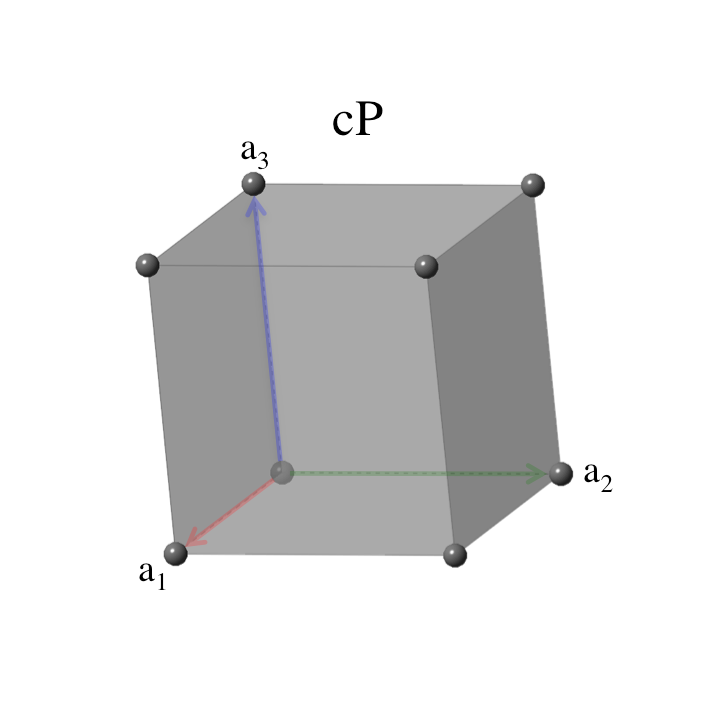
\includegraphics[width=3.5cm]{src/SC.png} & 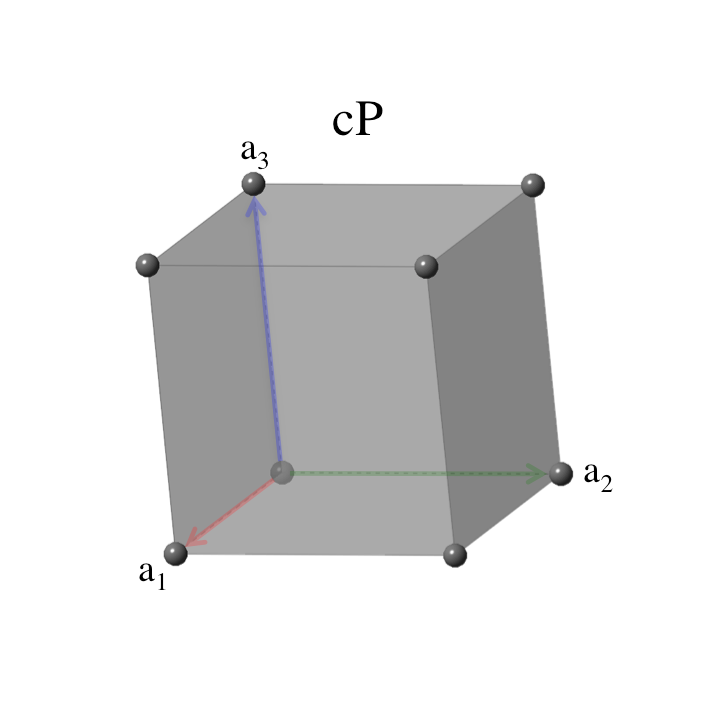
\includegraphics[width=3.5cm]{src/SC.png} & 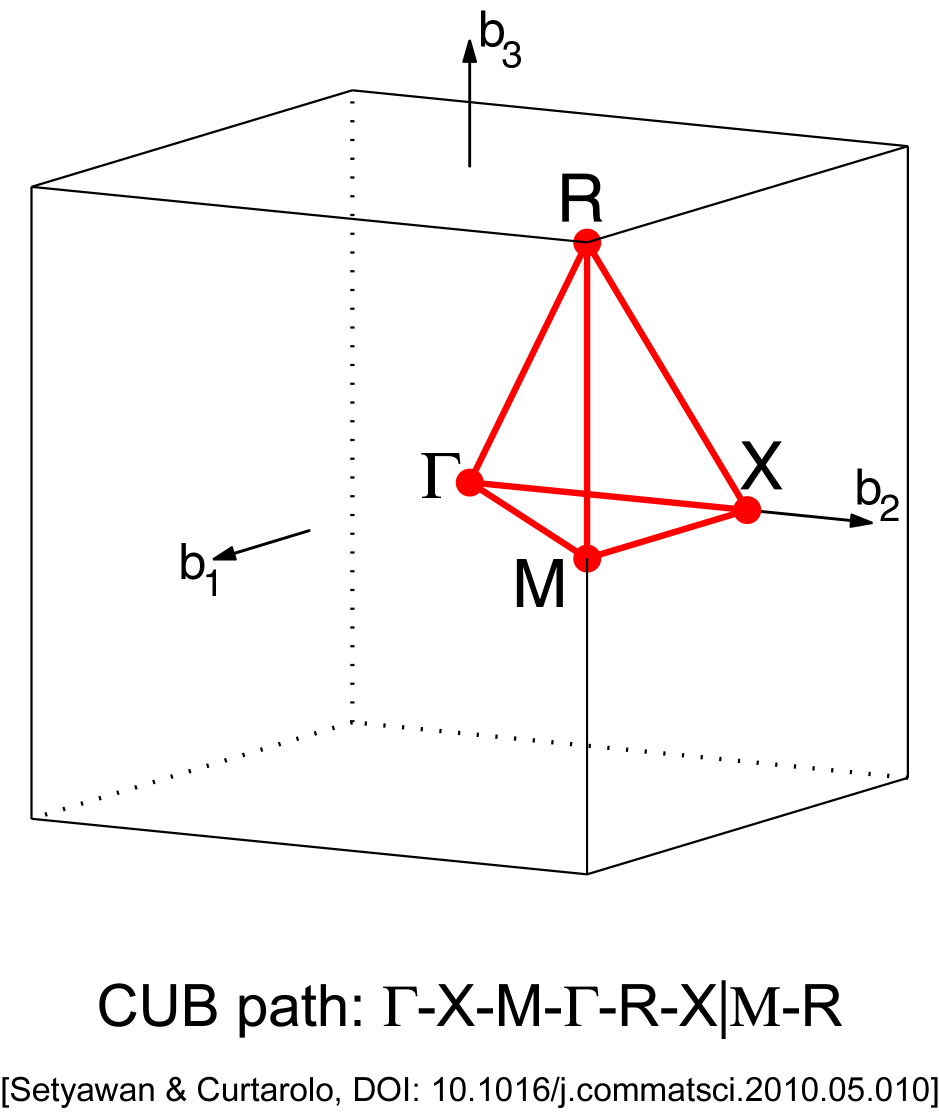
\includegraphics[width=3.5cm]{src/SCBZ.png} \\
        \hline
        \+:c1c{BCC} & \+:c1c{FCC,\ $V = 2\pare{\dfrac{2\pi}{a}}^3$} & \+:c1c{Rhombic Dodecahedron} \\
        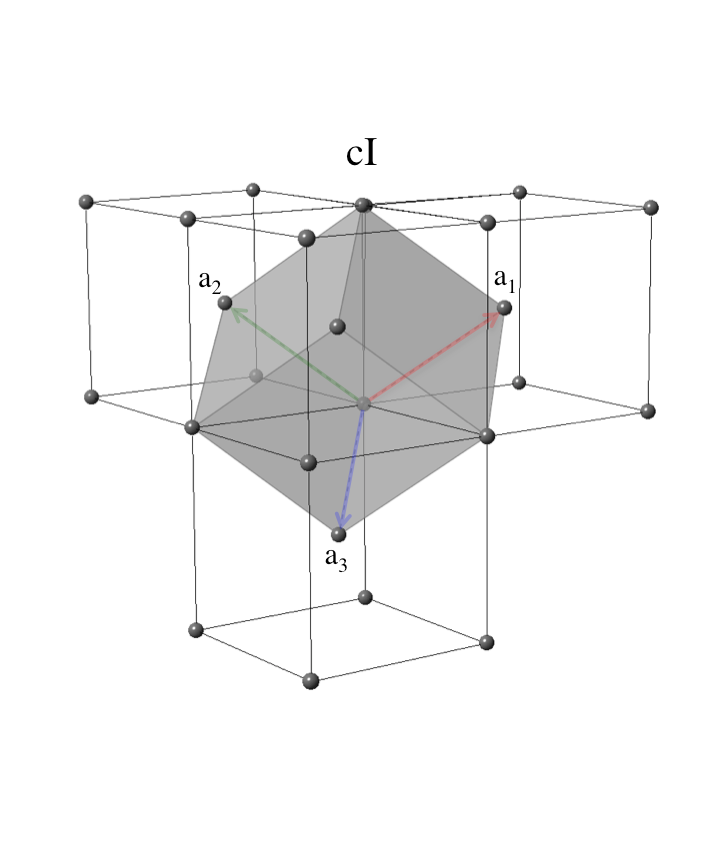
\includegraphics[width=3.5cm]{src/BCC.png} & 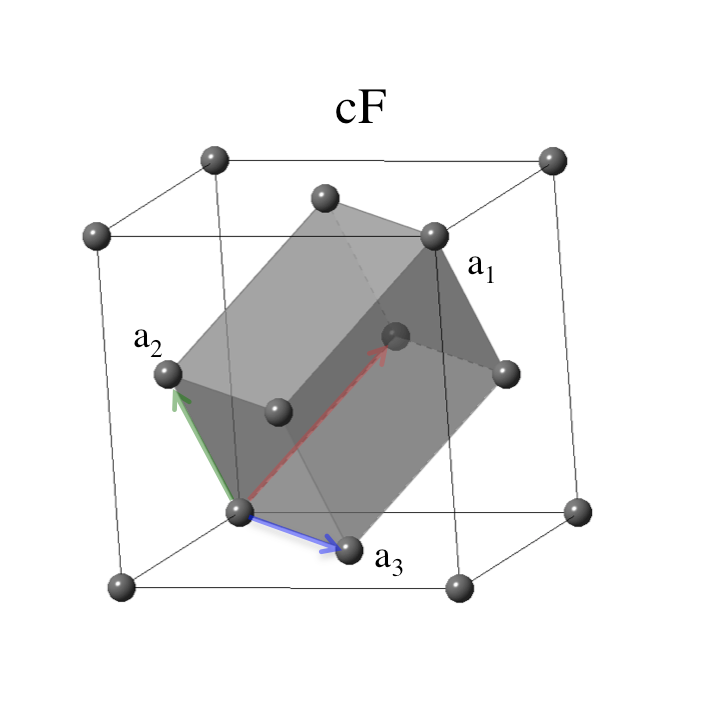
\includegraphics[width=3.5cm]{src/FCC.png} & 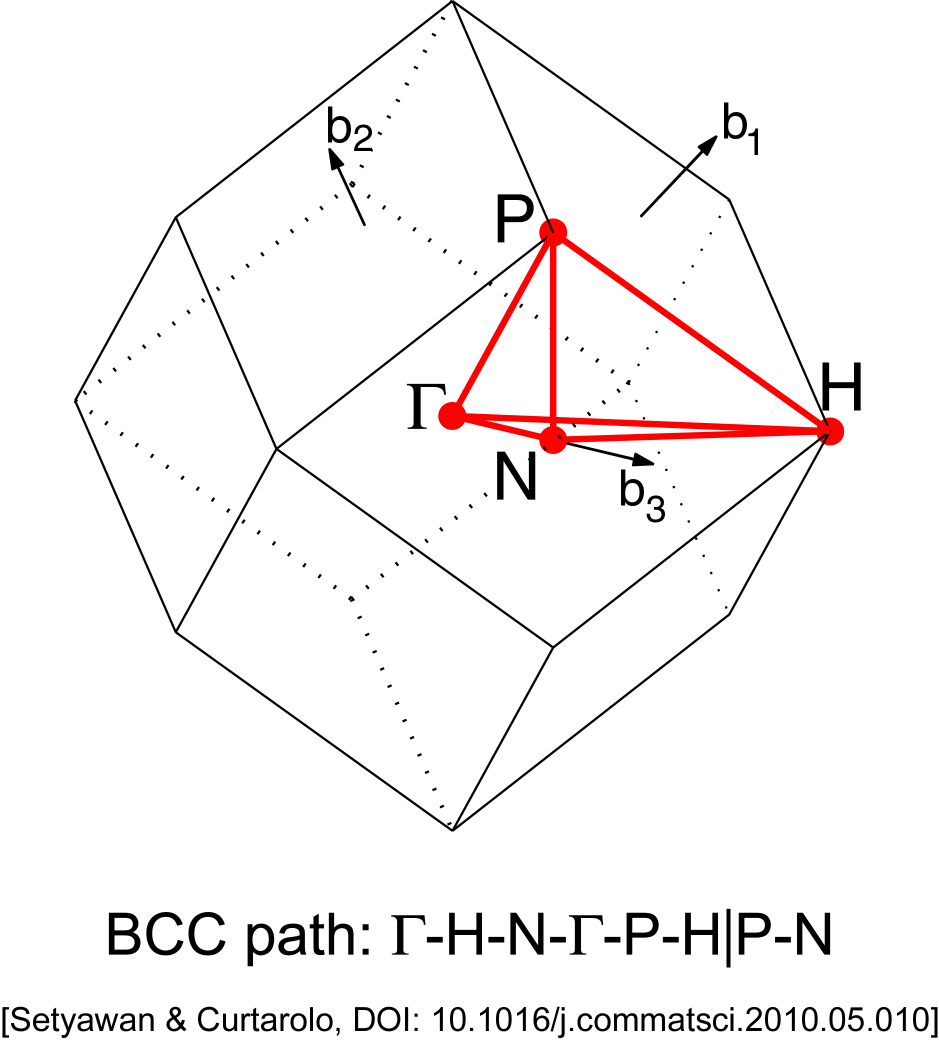
\includegraphics[width=3.5cm]{src/BCCBZ.png} \\
        \hline
        \+:c1c{FCC} & \+:c1c{BCC,\ $V = 4\pare{\dfrac{2\pi}{a}}^3$} & \+:c1c{Truncated Octahedron} \\
        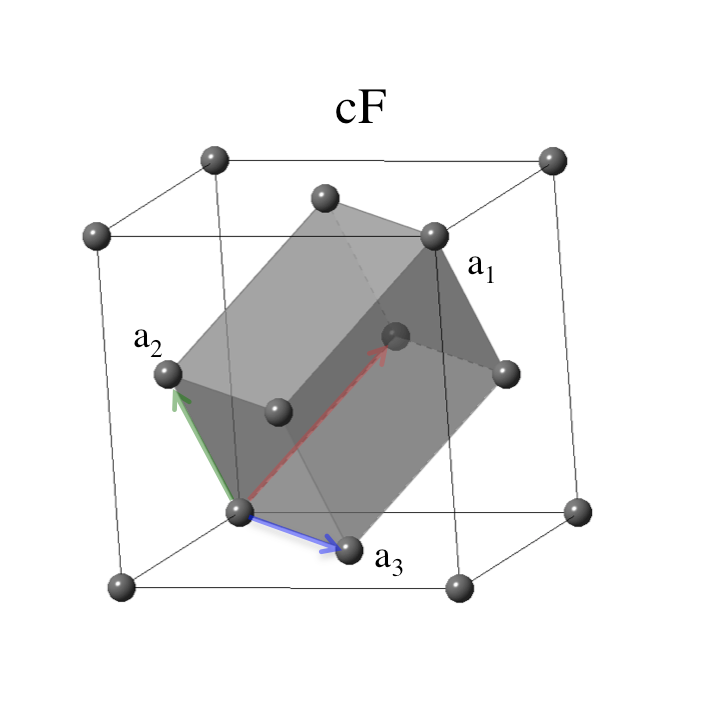
\includegraphics[width=3.5cm]{src/FCC.png} & 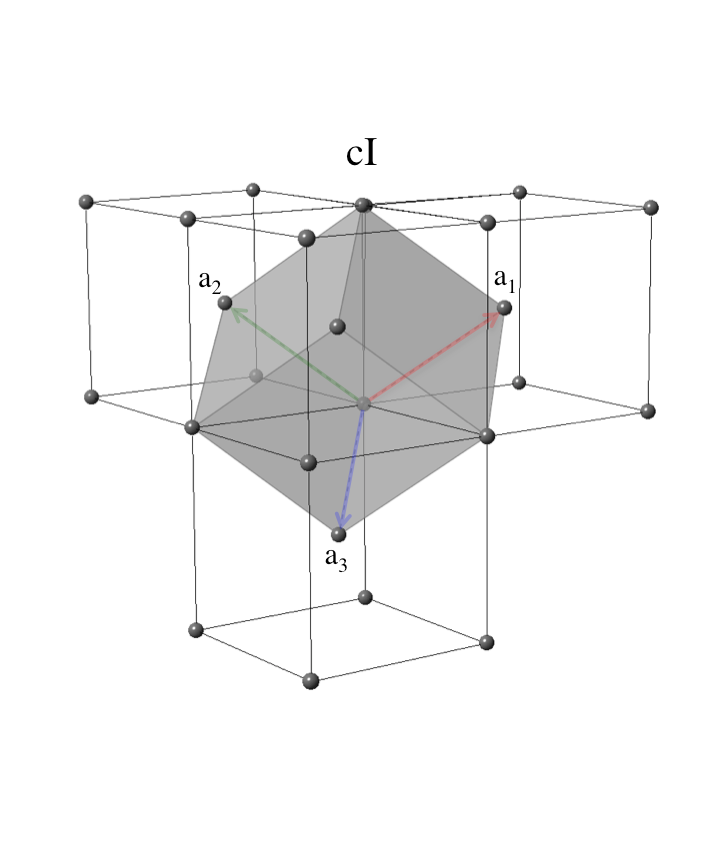
\includegraphics[width=3.5cm]{src/BCC.png} & 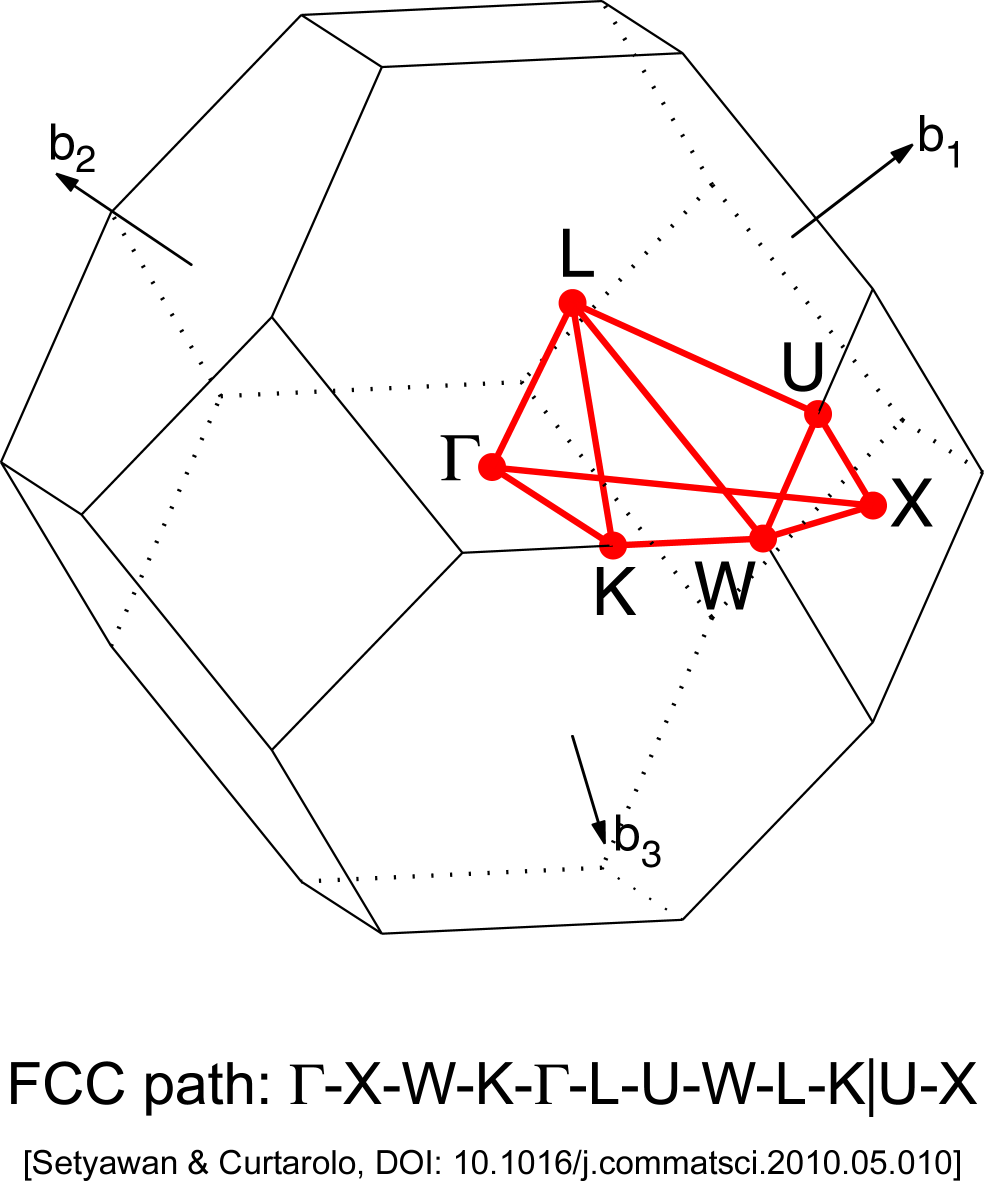
\includegraphics[width=3.5cm]{src/FCCBZ.png} \\
        \hline
    \end{tabular}
    \caption{The reciprocal lattices and the first Brillouin zones to the cubic crystal family.}
    \label{table:cubic_crystal_family}
\end{table}

% subsubsection brillouin_zones (end)

% subsection reciprocal_lattice (end)

\subsection{Diffaction} % (fold)
\label{sub:diffaction}

\subsubsection{Bragg's Law} % (fold)
\label{ssub:bragg_s_law}

\begin{figure}[ht]
    \centering
    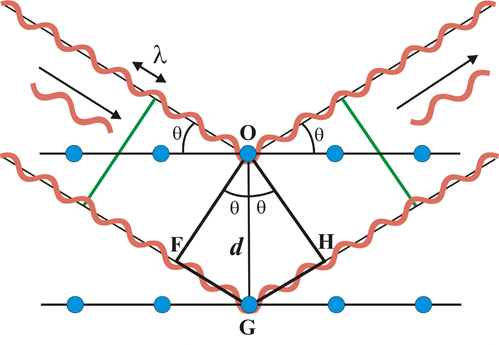
\includegraphics[width=6cm]{src/bragg.jpg}
    \caption{Bragg diffraction.}
    \label{fig:bragg_diffraction}
\end{figure}

\begin{finaleq}{Bragg's Law}
    Constructive interference occurs at those $\theta$ given by
    \[ 2d \sin\theta = n\lambda. \]
\end{finaleq}
Generally every lattice plane contribute \numrange{e-3}{e-5} of the total reflection amplitude.

% subsubsection bragg_s_law (end)

\subsubsection{Laue Equations} % (fold)
\label{ssub:laue_equations}

The amplitude of the scattered beam of wave vector $\+vk'$ is proportional to
\begin{equation}
    \label{eq:scattered_amplitude}
    F = \int \rd{V}\, n\pare{\+vr} e^{i\pare{\+vk - \+vk'}\cdot \+vr} = \int \rd{V}\, n\pare{\+vr} e^{-i\Delta \+vk\cdot \+vr} = \sum_{\+vG} \int \rd{V}\, n_{\+vG} e^{i\pare{\+vG - \Delta \+vk}\cdot \+vr},
\end{equation}
where $\+vk$ is the wave vector of the incident beam. The integral is taken on the whole crystal. $\inlinefinaleq{\Delta \+vk = \+vG}$ yields peaks of amplitude. For elastic scattering, where $\abs{\+vk} = \abs{\+vk'}$, the condition is written
\begin{finaleq}{Laue Equations}
    \[ \+vk\cdot \pare{\half \+vG} = \pare{\half G}^2,\quad \text{or}\quad \+va_i \cdot \Delta \+vk = 2\pi h_i,\quad \text{for}\quad i = 1,2,3, \]
    where the first equation is equivalent to saying that $\+vk$ lies on the bisector plane of a reciprocal lattice vector $\+vG$.
\end{finaleq}
With \eqref{eq:plane_distance} we find
\[ 2\cdot \frac{2\pi}{\lambda}\cdot \sin\theta = \frac{2\pi n}{d_{h_1h_2h_3}}, \]
i.e.
\[ 2d \sin\theta = n\lambda, \]
where $\theta$ is shown in \cref{fig:bragg_diffraction}.

% subsubsection laue_equations (end)

% subsection diffaction (end)

\subsection{Fourier Analysis of the Basis} % (fold)
\label{sub:fourier_analysis_of_the_basis}

\subsubsection{Structure Factors} % (fold)
\label{ssub:structure_factors}

When $\Delta \+vk = \+vG$, the scattered amplitude \eqref{eq:scattered_amplitude} is written
\[ F_{\+vG} = N\int\+_cell_ \rd{V}\, n\pare{\+vr} \exp\pare{-i\+vG\cdot \+vr} = NS_{\+vG}, \]
where $\+vr = 0$ at a corner of the cell, and $S_{\+vG}$ is called the \gloss[-2\baselineskip]{structure factor of the basis}.
\begin{termdef}{Atomic Form Factor}
    The atomic form factor is defined by
    \[ f_j = \int \rd{V}\, n_j\pare{\+v\rho} \exp\pare{-i\+vG\cdot \+v\rho}, \]
    integrated over all space, where $n$ is the charge density of the atom,
\end{termdef}
with which the structure factor of the basis may be written
\begin{finaleq}{The Structure Factor of the Basis}
    \[ S_{\+vG} = \sum_j f_j \exp\pare{-i\+vG\cdot \+vr_j} = \sum_j f_j \exp\brac{-2\pi i\pare{h_1 x_j + h_2 y_j + h_3 z_j}}, \]
\end{finaleq}
where $\pare{x_j,y_j,z_j}$ is the fractional coordinates of the atom.
\begin{sample}
    \begin{example}[Structure Factor of the BCC Lattice]
        \[ S_{\+vG} = f\curb{1+\exp\brac{-i\pi\pare{h_1 + h_2 + h_3}}} = \begin{cases}
            0, & \mathrm{if\ } h_1+h_2+h_3\mathrm{\ is\ odd}, \\
            2f, & \mathrm{if\ } h_1+h_2+h_3\mathrm{\ is\ even}. \\
        \end{cases} \]
    \end{example}
\end{sample}
\begin{sample}
    \begin{example}[Structure Factor of the FCC Lattice]
        \[ S_{\+vG} = f\curb{1+\exp\brac{-i\pi\pare{h_2 + h_3}}+\exp\brac{-i\pi\pare{h_1 + h_3}}+\exp\brac{-i\pi\pare{h_1 + h_2}}}. \]
        $S = 4f$ if the $h_j$ are all even or all odd. $S=0$ otherwise.
    \end{example}
\end{sample}

% subsubsection structure_factors (end)

\subsubsection{The Atomic Form Factor} % (fold)
\label{ssub:the_atomic_form_factor}

$\inlinefinaleq{f_j = Z_j}$ for \begin{margindef}{XRD}
    X-Ray Diffraction.
\end{margindef} spherically symmetric charge distributions located at $\+vr = 0$. This approximation works well for XRD.

% subsubsection the_atomic_form_factor (end)

% subsection fourier_analysis_of_the_basis (end)

% section crystal_diffraction_and_reciprocal_lattice (end)

\end{document}
